\documentclass[a4paper,12pt]{article}
\usepackage[utf8]{inputenc}
\usepackage{url}
\usepackage{epsfig}
\usepackage{graphics}
\usepackage{fancyhdr}

\graphicspath{{pictures/}}

\title{Sentence Generation using Two Models \\ \large{Final Project in the course DD2380 at KTH}}
\author{\hspace*{-0.5cm}
Group 61\\
\begin{tabular}{cccc}
K. Hannesson & J. Jóhannsson & E. Ahlsén & J. Andersson\\
Agust 20 & January 12 & BIRTHDATE3 & February 10 \\
hannesso@kth.se & jokull@kth.se & edvarda@kth.se & jonand8@kth.se \\
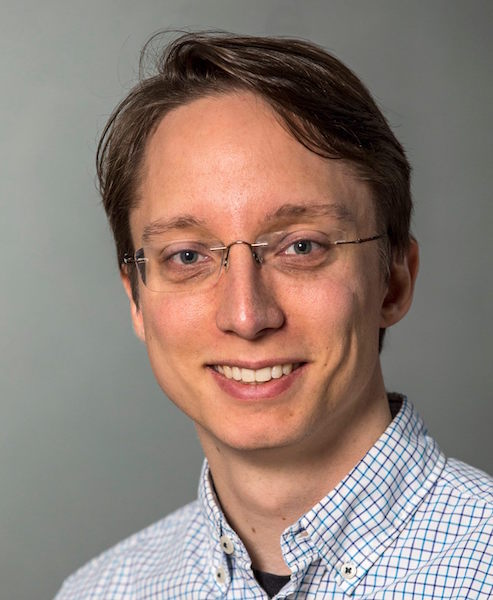
\includegraphics[width=0.13\linewidth]{photo_Kristofer} & 
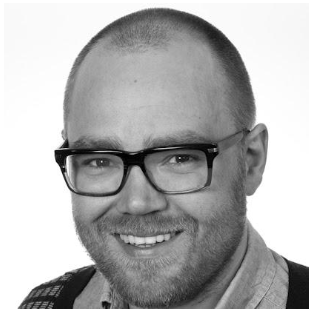
\includegraphics[width=0.13\linewidth]{photo_Jokull} & 
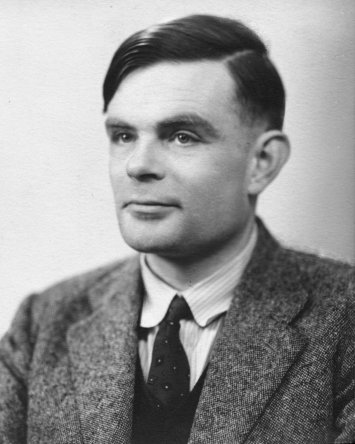
\includegraphics[width=0.13\linewidth]{Alan_Turing_photo} & 
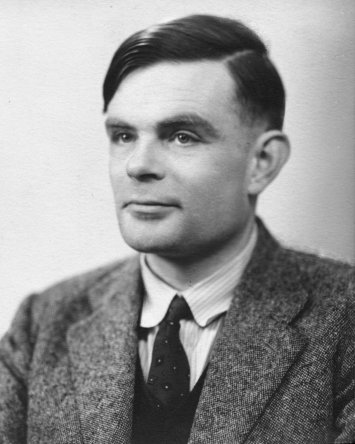
\includegraphics[width=0.13\linewidth]{Alan_Turing_photo}
\end{tabular}} 
% Normally there will not be any pictures but we want
% these so that we can connect faces to names in the course
% We also want birthdates so that we can tell people with the same
% name apart
\date{\today}

\pagestyle{fancy}
\setlength{\headheight}{15pt}
\fancyhf{}
\lhead{DD2380 ai15} % DO NOT REMOVE!!!!
\rhead{K. Hannesson, J. Jóhannsson, E. Ahlsén, J. Andersson} %% UPDATE WITH YOUR NAMES

\begin{document}

\maketitle
\thispagestyle{fancy}

\begin{abstract}
Bla bla bla bla bla bla bla bla bla bla bla bla bla bla bla bla bla 
bla bla bla bla bla bla bla bla bla bla bla bla bla bla bla bla bla 
bla bla bla bla bla bla bla bla bla bla bla bla bla bla bla bla bla 
bla bla bla bla bla bla bla bla bla bla bla bla bla bla bla bla bla
\end{abstract}



\clearpage

%%%%%%%%%%%%%%%%%%%%%%%%%%%%%%%%%%%%%%%%%%%%%%%%%%%%%%%%%%%%%
%%%%%%%%%%%%%%%%%%%%%%%%%%%%%%%%%%%%%%%%%%%%%%%%%%%%%%%%%%%%%
\section*{NOTE}
\begin{itemize}

\item The following sections are arranged in the order they would appear in a scientific paper. We think that these sections need to be there and written. However, these are only guidelines and if you think that some of these sections or subsections are irrelevant to you, please feel free to remove them. Similarly, if you want to include more sections or subsections please go ahead. Also feel free to rearrange them according to your convenience, but keeping some common sense (eg.~Introduction cannot come after Conclusions).

\item \textit{Introduction, Related Works, Experimental Results, Discussions, Summary} are sections that MUST be contained.

\item In the section of your \textit{Method}: please do not list your project as log book entries, please talk about the final method you want to present to us. Talk about the method scientifically or technically and not as "I did this..." "Then I tried this..." "this happened...." etc.

\item Do not paste any code unless it is very relevant!

\item The section \textit{Contributions} is a place to express any difference in contributions. The default assumption is that you all agree that all of you had an equal part to play in the project.

\item We suggest that you try to write this as scientifically as possible and not simply like a project report. Good Luck!

\item Please remove \textbf{this} NOTE section in your final report.

\end{itemize}
\section{Introduction (1--2 pages)}
\label{sec:intro}

Bla bla bla bla bla bla bla bla bla bla bla bla bla bla bla bla bla 
bla bla bla bla bla bla bla bla bla bla bla bla bla bla bla bla bla 
bla bla bla bla bla bla bla bla bla bla bla bla bla bla bla bla bla 
bla bla bla bla bla bla bla bla bla bla bla bla bla bla bla bla bla

\subsection{Contribution}
Bla bla bla bla bla bla bla bla bla bla bla bla bla bla bla bla bla 
bla bla bla bla bla bla bla bla bla bla bla bla bla bla bla bla bla 
bla bla bla bla bla bla bla bla bla bla bla bla bla bla bla bla bla 
bla bla bla bla bla bla bla bla bla bla bla bla bla bla bla bla bla

\subsection{Outline}
Bla bla bla bla bla bla bla Section~\ref{sec:relwork} bla bla bla bla 
bla bla bla bla bla Section~\ref{sec:method} bla bla bla bla bla bla 
bla bla bla bla bla bla bla bla bla bla bla Section~\ref{sec:exps}
bla bla bla bla bla bla Section~\ref{sec:summary} bla bla bla bla bla

%%%%%%%%%%%%%%%%%%%%%%%%%%%%%%%%%%%%%%%%%%%%%%%%%%%%%%%%%%%%%
%%%%%%%%%%%%%%%%%%%%%%%%%%%%%%%%%%%%%%%%%%%%%%%%%%%%%%%%%%%%%
\section{Related work}
\label{sec:relwork}

Bla bla bla bla bla bla bla bla bla bla bla bla bla bla bla bla bla 
bla bla bla bla bla bla bla bla bla bla bla bla bla bla bla bla bla 
bla bla bla bla bla bla bla bla bla bla bla bla bla bla bla bla bla 
bla bla bla bla bla bla bla bla bla bla \cite{RussellNorvigAIBook3rd}
bla bla bla bla bla bla

%%%%%%%%%%%%%%%%%%%%%%%%%%%%%%%%%%%%%%%%%%%%%%%%%%%%%%%%%%%%%
%%%%%%%%%%%%%%%%%%%%%%%%%%%%%%%%%%%%%%%%%%%%%%%%%%%%%%%%%%%%%
\section{Our method}
\label{sec:method}

The group came up with the idea to compare two different approaches to generating text from a corpus, both including grammar but in different ways. To be able to compare them at the same level both approaches used the Brown corpus and trigrams, with fallback to bigrams allowed. A few smoothing techniques were picked for use in both approaches.

The first approach was to create a model that included both word and grammar information. This was achieved by generating trigrams where each word was a tuple of the word and its associated Part-Of-Speech (POS) tag. A trigram from ``the man walked'' would be (the, DET), (man, NOUN), (walked, VERB)) 

The second approach separated grammar and words into two models which were used in sequence to generate text. The grammar model provided what POS tag should be next, and the word model provided a word for the given tags, both using trigrams. This would take ``the man walked'' and create the trigrams (DET, NOUN, VERB) for the grammar model, and (DET, NOUN, man) and (NOUN, VERB, walked) for the grammar-word model.

The smoothing techniques chosen were:
\begin{itemize}
\item Maximum Likelihood Estimate
\item Laplace smoothing
\item Expected Likelihood Estimate
\item Simplified Good-Turing Frequency Estimation
\end{itemize}

\subsection{Implementation}
\label{sec:impl}

We split into pairs with each pair implementing their model. We decided to go with Python 3 for the implementation because we knew the NLTK package would provide us with the necessary building blocks to construct and test the two models. These included 
\begin{itemize}
\item Brown corpus
\item Treebank Part of Speech Tagger (Maximum entropy)
\item Punkt Tokenizer Models
\item Mappings to the Universal Part-Of-Speech Tagset
\item Conditional Frequency Distribution and Conditional Probability Distribution classes
\item classes for each of the above mentioned smoothing techniques
\end{itemize}



  

%%%%%%%%%%%%%%%%%%%%%%%%%%%%%%%%%%%%%%%%%%%%%%%%%%%%%%%%%%%%%
%%%%%%%%%%%%%%%%%%%%%%%%%%%%%%%%%%%%%%%%%%%%%%%%%%%%%%%%%%%%%
\section{Experimental results}
\label{sec:exps}

Bla bla bla bla bla bla bla bla bla bla bla bla bla bla bla bla bla 
bla bla bla bla bla bla bla bla bla bla bla bla bla bla bla bla bla 
bla bla bla bla bla bla bla bla bla bla bla bla bla bla bla bla bla 

\subsection{Experimental setup}
Each model was used to generate 5 sentences per smoothing method for a total of 40 sentences. 5 sentences were also picked from the Brown corpus. All the sentences were mixed together randomly and then added to a survey which allowed participants to rate each sentence on a scale of 1 to 5 whether it was created by a human or a computer, with 1 representing definitely a human and 5 definitely a computer. Apart from the sentence scoring we only asked if the participants were native English speakers or not. The survey solution chosen was QuestionPro.

\subsection{Experiment ...}

Bla bla bla bla bla bla bla bla bla bla bla bla bla bla bla bla bla 
bla bla bla bla bla bla bla bla bla bla bla bla bla bla bla bla bla 
bla bla bla bla bla bla bla bla bla bla bla bla bla bla bla bla bla 

\begin{figure}
\centering
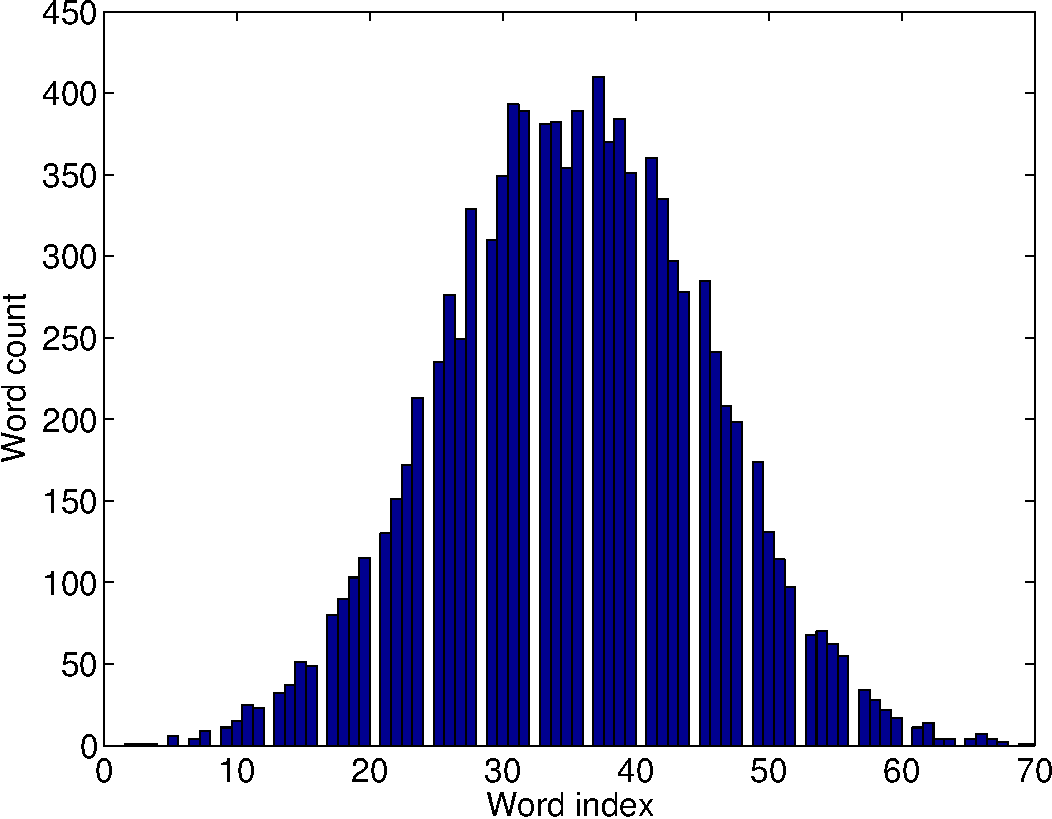
\includegraphics[width=0.8\linewidth]{histogram}
\caption{A description that makes browsing the paper easy and clearly 
describes what is in the picture. Make sure that the text in the figure 
is large enough to read and that the axes are labelled.}
\label{fig:histogram}
\end{figure}

Bla bla bla bla bla Figure~\ref{fig:histogram} bla bla bla bla bla bla 
bla bla bla bla bla bla bla bla bla bla bla bla bla bla bla bla bla 
bla bla bla bla bla bla bla bla bla bla bla bla bla bla bla bla bla 

\begin{table}
\begin{center}
\begin{tabular}{|c|c|c|}
\hline
Bla bla & Bla bla & Bla bla \\ \hline
42 & 42 & 42 \\ \hline
42 & 42 & 42 \\ \hline
\end{tabular}
\caption{A description that makes browsing the paper easy and clearly 
describes what is in the table.}
\label{tab:results}
\end{center}
\end{table}

Bla bla bla bla bla Table~\ref{tab:results} bla bla bla bla bla bla 
bla bla bla bla bla bla bla bla bla bla bla bla bla bla bla bla bla 
bla bla bla bla bla bla bla bla bla bla bla bla bla bla bla bla bla 

%%%%%%%%%%%%%%%%%%%%%%%%%%%%%%%%%%%%%%%%%%%%%%%%%%%%%%%%%%%%%
%%%%%%%%%%%%%%%%%%%%%%%%%%%%%%%%%%%%%%%%%%%%%%%%%%%%%%%%%%%%%
\section{Summary and Conclusions}
\label{sec:summary}

Bla bla bla bla bla bla bla bla bla bla bla bla bla bla bla bla bla 
bla bla bla bla bla bla bla bla bla bla bla bla bla bla bla bla bla 
bla bla bla bla bla bla bla bla bla bla bla bla bla bla bla bla bla 


%%%%%%%%%%%%%%%%%%%%%%%%%%%%%%%%%%%%%%%%%%%%%%%%%%%%%%%%%%%%%
%%%%%%%%%%%%%%%%%%%%%%%%%%%%%%%%%%%%%%%%%%%%%%%%%%%%%%%%%%%%%
\section{Contributions}
\label{sec:contributions}
We the members of project group 61 unanimously declare that 
we have all equally contributed toward the completion of this
project.

%%%%%%%%%%%%%%%%%%%%%%%%%%%%%%%%%%%%%%%%%%%%%%%%%%%%%%%%%%%%%
%%%%%%%%%%%%%%%%%%%%%%%%%%%%%%%%%%%%%%%%%%%%%%%%%%%%%%%%%%%%%
\bibliographystyle{plain}
\bibliography{reflist}


\end{document}